%
%  Erik Olsen
%
\documentclass[12pt,fullpage]{article}
\usepackage{fullpage}                                        % use all of the page for text 
\usepackage{psfrag}                                          % LaTeX graphics tool
\usepackage{pslatex}                                         % avoids the default cmr font
\usepackage{graphicx}                                        % graphics package 
\usepackage{epsfig}                                          % figures
\usepackage{epsfig} 
\usepackage{hyperref}
\usepackage{color}

\begin{document}

\noindent
{\bf Lomax Distribution} (from \color{blue}\url{http://www.math.wm.edu/~leemis/chart/UDR/UDR.html}\color{black})

\noindent
The shorthand $X \sim {\rm Lomax}(\lambda, \kappa)$ is used to indicate that the
random variable $X$ has the Lomax distribution with parameters $\lambda$ and $\kappa$.
A Lomax random variable $X$ with scale parameter $\lambda$ and shape parameter $\kappa$ 
has probability density function 
$$
f(x) = \frac{\lambda \kappa} {\left( 1 + {\lambda}\,x \right) ^{\kappa + 1}} \qquad \qquad x > 0,
$$  
for $\lambda > 0$ and $\kappa>0$.\\
The probability density function with two different parameterizations is illustrated below:
{\begin{figure}[h!]
\begin{center}
\psfrag{lab1}{$\lambda \kern -0.08 em = \kern -0.08 em  1,\, \kappa \kern -0.08 em  = \kern -0.08 em  1$}
\psfrag{lab2}{$\lambda \kern -0.08 em  = \kern -0.08 em  1,\, \kappa \kern -0.08 em  = \kern -0.08 em  5$}
\psfrag{labx}{$x$}
\psfrag{labf}{$f(x)$}
\includegraphics[width=3.2in]{LomaxPlot.ps}
\end{center}
\end{figure}}\\
Using the original parameterization, the cumulative distribution function on
the support of $X$ is
$$
F(x) = P(X \le x) = 1 - \left( 1 + {\lambda}\,x \right) ^ {-{\kappa}}  \qquad  \qquad  x > 0.
$$
The survivor function on the support of $X$ is
$$
S(x) = P(X \ge x) = \left(1 + \lambda\, x\right) ^ {-\kappa}  \qquad \qquad x > 0.
$$
The hazard function on the support of $X$ is
$$
h(x) = \frac{f(x)}{S(x)} = \frac{\lambda \kappa} {1 + \lambda x}  \qquad \qquad x > 0.
$$
The cumulative hazard function on the support of $X$ is
$$
H(x) = - \ln \kern 0.04em S(x) = \kappa \kern 0.04em \ln(1 + \lambda \,x)  \qquad \qquad x > 0.
$$
The inverse distribution function of $X$ is
$$
F ^ {-1}(u) = \frac{\left(1 - u\right) ^ {-1 /  \kappa} - 1}{\lambda}  \qquad \qquad 0 < u < 1.
$$
The median of $X$ is
$$
\frac{2^{1/\kappa} - 1}{\lambda}.
$$
The moment generating function of $X$ is mathematically intractable.
The population mean of $X$ is 
$$
E[X]=\frac{\lambda}{\kappa - 1}$$ provided $\kappa > 1$. The population variance, skewness, and kurtosis of $X$ are mathematically intractable.\\
For $X_1, \, X_2, \, \ldots , \, X_n$ mutually independent Lomax($\lambda$) random variables,
the maximum likelihood estimator for $\alpha$ is
$$
\hat \alpha = \frac{n}{\sum_{i=1} ^ n \ln\left(1 +  x_i  /  \hat\lambda \right)}.
$$
An iteration procedure must be used to solve the following equation for $\hat\lambda$, and then substitute in the previous to obtain $\hat\alpha$.
$$
\frac{n}{\hat\lambda\left(\sum_{i=1} ^ n \frac{x_i}{\hat\lambda^2 + \hat\lambda x_i}\right)} - 1 = \frac{n}{\sum_{i=1} ^ n \ln\left(1 + \frac{x_i}{\hat\lambda}\right)}
$$ 


\vspace{0.1in}

\noindent
%{\bf APPL results:}
%The APPL statements
%\begin{verbatim}
%X := LomaxRV(kappa, lambda);
%CDF(X);
%Mean(X);
%Variance(X);
%Skewness(X);
%Kurtosis(X);
%MGF(X);
%\end{verbatim}
%result in the cumulative distribution function, population mean, variance, skewness, kurtosis, and moment generating function.

\end{document}
